%%%%%%%%%%%%%%%%%%%%%%%%%%%%%%%%%%%%%%%%%%%%%%%%%%%%%%%%%%%%%%%%%%%%%
%
%   Presentation for:
%
%   Workshop on Adaptive Filters in Bucure\c{s}ti / Romania
%   (March 2003)
%
%   (c) Matthias M\"{u}hlich, 03/2003
%
%%%%%%%%%%%%%%%%%%%%%%%%%%%%%%%%%%%%%%%%%%%%%%%%%%%%%%%%%%%%%%%%%%%%%



% this file must be processed with pdflatex!



\documentclass[english,pdftex]{article}

\usepackage{babel}          %% hyphenation patterns - takes global option english
\usepackage{palatino}       %% Palatino fonts
\usepackage{mathptm}        %% PostScript Type 1 math fonts
\usepackage{textcomp}       %% symbols
\usepackage[paneltoc,sectionbreak]{pdfwin}  %% my presentation style file
                                            %% takes global options english + pdftex



% character protruding; disabled for higher compatibility
%\pdfprotrudechars=2

\lpcode`\(=50 \lpcode`\A=50 \lpcode`\J=50 \lpcode`\T=50
\lpcode`\V=50 \lpcode`\W=50 \lpcode`\X=50 \lpcode`\Y=50
\lpcode`\v=50 \lpcode`\w=50 \lpcode`\x=50 \lpcode`\y=50
\rpcode`\-=700 \rpcode`\.=700 \rpcode`\,=700 \rpcode`\�=700
\rpcode`\;=500 \rpcode`\:=500 \rpcode`\!=200 \rpcode`\?=200
\rpcode`\)=50 \rpcode`\A=50 \rpcode`\F=50 \rpcode`\K=50
\rpcode`\L=50 \rpcode`\T=50 \rpcode`\V=50 \rpcode`\W=50
\rpcode`\X=50 \rpcode`\Y=50 \rpcode`\k=50 \rpcode`\r=50
\rpcode`\t=50 \rpcode`\v=50 \rpcode`\w=50 \rpcode`\x=50
\rpcode`\y=50


% abbreviation for vectors
% shortvec.tex -- abbreviation for vectors

% matrices
\newcommand{\mat}[1]{\mathbf{#1}}
\newcommand{\MA}{\mat{A}} \newcommand{\MB}{\mat{B}} \newcommand{\MC}{\mat{C}}
\newcommand{\MD}{\mat{D}} \newcommand{\ME}{\mat{E}} \newcommand{\MF}{\mat{F}}
\newcommand{\MG}{\mat{G}} \newcommand{\MH}{\mat{H}} \newcommand{\MI}{\mat{I}}
\newcommand{\MJ}{\mat{J}} \newcommand{\MK}{\mat{K}} \newcommand{\ML}{\mat{L}}
\newcommand{\MM}{\mat{M}} \newcommand{\MN}{\mat{N}} \newcommand{\MO}{\mat{O}}
\newcommand{\MP}{\mat{P}} \newcommand{\MQ}{\mat{Q}} \newcommand{\MR}{\mat{R}}
\newcommand{\MS}{\mat{S}} \newcommand{\MT}{\mat{T}} \newcommand{\MU}{\mat{U}}
\newcommand{\MV}{\mat{V}} \newcommand{\MW}{\mat{W}} \newcommand{\MX}{\mat{X}}
\newcommand{\MY}{\mat{Y}} \newcommand{\MZ}{\mat{Z}} \newcommand{\Mnull}{\mat{0}}

% vectors
\newcommand{\va}{\vec a} \newcommand{\vb}{\vec b} \newcommand{\vc}{\vec c}
\newcommand{\vd}{\vec d} \newcommand{\ve}{\vec e} \newcommand{\vf}{\vec f}
\newcommand{\vg}{\vec g} \newcommand{\vh}{\vec h} \newcommand{\vi}{\vec i}
\newcommand{\vj}{\vec j} \newcommand{\vk}{\vec k} \newcommand{\vl}{\vec l}
\newcommand{\vm}{\vec m} \newcommand{\vn}{\vec n} \newcommand{\vo}{\vec o}
\newcommand{\vp}{\vec p} \newcommand{\vq}{\vec q} \newcommand{\vr}{\vec r}
\newcommand{\vs}{\vec s} \newcommand{\vt}{\vec t} \newcommand{\vu}{\vec u}
\newcommand{\vv}{\vec v} \newcommand{\vw}{\vec w} \newcommand{\vx}{\vec x}
\newcommand{\vy}{\vec y} \newcommand{\vz}{\vec z}

% EOF




% SETUP OF PDFWIN PACKAGE
%
% define windows and margins
\SetScreen{width=12cm, height=9cm}
\SetWindow{text}{basex=0.2cm, basey=0.2cm, width=9.4cm,height=8.6cm,
borderthickness=0.4mm}
\SetWindow{panel}{basex=9.8cm, basey=0.2cm, width=2cm,
height=8.6cm, borderthickness=0.4mm}
\SetButtons{width=1.6cm, shadowdepth=0.3mm}
\SetMargins{.5cm}{.5cm}{.5cm}{.5cm}
%
% define panel
\SetLogo{filename=JWGU-Logo.png,width=1.3cm, shadowdepth=.7mm}
\SetScreen{type=wallpaper, filename=marble.png}
\SetPaneltext{\scriptsize\sffamily Filter-Workshop\\Bucure\c{s}ti
2003}
\renewcommand{\DrawNavigationPanel}{
  \ShowPageInfo\par\vfill
  \FirstLastButton\par\vfill
  \PrevNextButton\par\vfill
  \BackForwardButton\par\vfill
  \FullScreenButton\par\vfill
  \SearchButton\par\vfill
  \CloseButton\par\vfill
}


% COLORS
%
% windows
\definecolor{titlecolor}{rgb}{.7,.15,.1}
\definecolor{TextBackgroundColor}{rgb}{.7,.8,1.0}
\definecolor{TextBorderColor}{rgb}{0,0,.5}
%
% colors for presentation
\definecolor{StateColor}{rgb}{0,0,.6}
\definecolor{StateFuncColor}{rgb}{.4,0,.3}
\definecolor{StateNoiseColor}{rgb}{.3,.3,.7}
\definecolor{MeasColor}{rgb}{0,.5,0}
\definecolor{MeasFuncColor}{rgb}{.4,.3,0}
\definecolor{MeasNoiseColor}{rgb}{.3,.7,.3}
\definecolor{InputColor}{rgb}{.7,0,0}
%
% colors for environments
\definecolor{CodeTextColor}{rgb}{0,0.3,0}
\definecolor{CodeMathColor}{rgb}{0.1,0.3,0.6}
\definecolor{MyBoxColor1}{rgb}{.8,.5,.1}
\definecolor{MyBoxColor2}{rgb}{.9,.8,.3}
\definecolor{MyBoxiiColor1}{rgb}{.8,.6,.4}
\definecolor{MyBoxiiColor2}{rgb}{.9,.8,.7}
\definecolor{MyCodeBoxColor1}{rgb}{.3,.6,.2}
\definecolor{MyCodeBoxColor2}{rgb}{.8,.9,.7}
%
% misc
\definecolor{dgreen}{rgb}{0,.6,0}


% LAYOUT
%
% general layout
\tolerance=2000
\emergencystretch=5em
\fboxsep=3mm
\setlength{\parskip}{4pt plus 2pt minus 1pt}
\setlength{\parindent}{0pt}
\frenchspacing
%
% define page transition style
\pdfpageattr{/Trans << /S /Dissolve /D 0.3 >>}
%
% replace default font (roman default) by computer modern sans serif;
% Palatino only for panel
% NOTE: brute force, no good style here...
\renewcommand{\rmdefault}{cmss}
%
% redefine vector style (boldface instead of arrow on top)
\renewcommand{\vec}[1]{\mathbf{#1}}
%
% redefine section numbering: only section (and no subsection or lower)
% gets a number
\setcounter{secnumdepth}{1}


% NEW COMMANDS
%
\newcommand{\Realnumbers}{\mathrm{I\!R}}
\newcommand{\Expect}[1]{\mbox{{\sf E}}\left[ #1 \right]}
\newcommand{\Cov}[1]{\mbox{\sf Cov}\left[ #1 \right]}
%
\newcommand{\mybox}[1]{\begin{center}%
  \fboxrule=.5mm%
  \fcolorbox{MyBoxColor1}{MyBoxColor2}{%
  \parbox[c]{.9\textwidth}{#1}}%
\end{center}}
%
\newcommand{\myboxii}[1]{\begin{center}%
  \fboxrule=.5mm%
  \fcolorbox{MyBoxiiColor1}{MyBoxiiColor2}{%
  \parbox[c]{.9\textwidth}{#1}}%
\end{center}}
%
\newcommand{\mycodebox}[1]{\begin{center}%
  \fboxrule=.5mm%
  \ttfamily\bfseries%
  \color{CodeTextColor}%
  \fcolorbox{MyCodeBoxColor1}{MyCodeBoxColor2}{%
  \parbox[c]{.9\textwidth}{#1}}%
\end{center}}
%
\newcommand{\codemath}[1]{\textcolor{CodeMathColor}{$#1$}}
\newcommand{\codetext}[1]{\textsf{\mdseries\small #1}}



%====================================================================



\begin{document}



% produce panel TOC entry for title page
\AddPanelTocEntry{Title Page}%

{\centering {\Huge\bfseries\color{titlecolor}
  Particle Filters\rule[-.6ex]{0pt}{5ex}\\
  \LARGE an overview\rule[-.6ex]{0pt}{3ex}\\
} \vspace*{8mm}
{\Large Matthias M\"{u}hlich}\\[3ex]
  \large Institut f{\"u}r Angewandte Physik\\
        J.W.Goethe-Universit{\"a}t Frankfurt\\
  \href{mailto:muehlich@iap.uni-frankfurt.de}{\color{black}muehlich@iap.uni-frankfurt.de}\\
}




\newpage

% replacement title page
{\centering {\Huge\bfseries\color{titlecolor}
  Particle Filters\rule[-.6ex]{0pt}{5ex}\\
  \LARGE a tutorial\rule[-.6ex]{0pt}{3ex}\\
} \vspace*{8mm}
{\Large Matthias M\"{u}hlich}\\[3ex]
  \large Institut f{\"u}r Angewandte Physik\\
        J.W.Goethe-Universit{\"a}t Frankfurt\\
  \href{mailto:muehlich@iap.uni-frankfurt.de}{\color{black}muehlich@iap.uni-frankfurt.de}\\
}




\section{Introduction}
\label{Intro}

% change text window style from normal (-> title page) to transparent
% (-> rest of talk); must appear after page break, i.e. section command
% ("sectionbreak" option for pdfwin produces page break at each \section
% command)
\SetWindow{text}{type=transparent, borderthickness=0.5mm}


An increasing number of researchers is using a family of
techniques and algorithms called
\begin{itemize}
\itemsep=-1mm
    \item \textit{condensation algorithms}
    \item \textit{bootstrap filtering}
    \item \textit{particle filters}
    \item \textit{interacting particle approximations}
    \item \textit{sequential Monte Carlo methods}
    \item \textit{SIS, SIR, ASIR, RPF, \dots}
\end{itemize}
Time scale: last 10 years [e.g. Isard \& Blake 1996; Kitagawa
1996; Gordon, Salmond \& Smith 1993]
%
\mybox{The question of this talk is: What is behind all that?}



\newpage
\subsection{General Classification of %On-line
Filter Strategies}

Gaussian models:
\begin{itemize}
   \item Kalman filter
   \item extended Kalman filter
   \item linear-update filter / linear regression filter /\\
      statistical linearization filter
   \begin{itemize}
      \item unscented filter
      \item central difference filter
      \item divided difference filter
   \end{itemize}
   \item assumed density filter / moment matching
\end{itemize}

\newpage
Mixture of Gaussian models:
\begin{itemize}
   \item assumed density filter / pseudo-Bayes
   \item Gaussian-sum filter
\end{itemize}

\bigskip
Nonparametric models:
\begin{itemize}
   \item \textcolor{red}{\bfseries particle filter class}
   \item histogram filter
\end{itemize}


\newpage
\subsection{Some Basic Remarks}

\begin{itemize}
  \item various applications: computer vision (i.e. tracking),
  control theory, econometrics (stock markets, monetary flow, interest
  rates), \dots
  \item we deal with discrete time systems only
  \item no out-of-sequence measurements
  \item we are mainly interested in estimating the state at time
  $k$ from measurements up to time $k'=k$ (opposite: smoothing
  ($k'>k$) and prediction ($k'<k$); furthermore $k'$ need not be
  fixed\dots)
  \item no restrictions to linear processes or Gaussian noise!
\end{itemize}


\inithighlight{\subsection*{Overview of this Talk}
\begin{center}
\begin{itemize}
\item
    {\color{color1} The Dynamic System Model}
\item
    {\color{color2} Bayesian Filter Approach}
\item
    {\color{color3} Optimal and Suboptimal Solutions}
\item
    {\color{color4} The Particle Filter}
\item
    {\color{color5} Experiments and Summary}
\end{itemize}
\end{center}
\vspace{4mm} }


\highlightnext
\pagenumbering{incremental}

-- states of a system and state transition equation

-- measurement equation


\highlightnext

-- estimation of the state

-- probabilistic modelling

-- Bayesian filter


\highlightnext

-- filtered pdf can be written down easily, but it is not always
tractable ($\rightarrow$ ugly integrals \dots)

-- conditions under which optimal solutions exist: Kalman filter
and grid-based filter

-- what can be done in other cases: suboptimal approaches


\highlightnext

-- standard particle filter

-- various improved versions


\highlightnext

-- some experimental data and conclusion



\newpage
\pagenumbering{restore}


\section{Dynamic System}

A dynamic system can be modelled with two equations:

\subsection{State Transition or Evolution Equation}
 \[
    {\color{StateColor}\vx_k} = {\color{StateFuncColor}f_k}({\color{StateColor}\vx_{k-1}},
    {\color{InputColor}\vu_{k-1}},{\color{StateNoiseColor}\vv_{k-1}})
 \]

${\color{StateFuncColor}f}(\cdot,\cdot,\cdot)$:
{\color{StateFuncColor}evolution
function} (possible non-linear) \\
${\color{StateColor}\vx_k}, {\color{StateColor}\vx_{k-1}} \in
\Realnumbers^{n_x}$:
current and previous {\color{StateColor}state} \\
${\color{StateNoiseColor}\vv_{k-1}} \in \Realnumbers^{n_v}$:
{\color{StateNoiseColor}state noise}
(usually \emph{not} Gaussian)\\
${\color{InputColor}\vu_{k-1}} \in
\Realnumbers^{n_u}$: known {\color{InputColor}input}

\bigskip
Note: state only depends on previous state, i.e. first order
Markov process




\newpage
\subsection{Measurement Equation}
 \[
    {\color{MeasColor}\vz_k} = {\color{MeasFuncColor}h_k}({\color{StateColor}\vx_k},
    {\color{InputColor}\vu_k},{\color{MeasNoiseColor}\vn_k})
 \]

${\color{MeasFuncColor}h}(\cdot,\cdot,\cdot)$:
{\color{MeasFuncColor}measurement
function} (possible non-linear) \\
${\color{MeasColor}\vz_k} \in
\Realnumbers^{n_z}$: {\color{MeasColor}measurement} \\
${\color{StateColor}\vx_k} \in
\Realnumbers^{n_x}$: {\color{StateColor}state} \\
${\color{MeasNoiseColor}\vn_k} \in \Realnumbers^{n_n}$:
{\color{MeasNoiseColor}measurement noise}
(usually \emph{not} Gaussian)\\
${\color{InputColor}\vu_k} \in
\Realnumbers^{n_u}$: known {\color{InputColor}input}

\bigskip
(dimensionality of {\color{StateColor}state},
{\color{MeasColor}measurement}, {\color{InputColor}input},
{\color{StateNoiseColor}state noise}, and
{\color{MeasNoiseColor}measurement noise} can all be different!)




\newpage
\pagenumbering{incremental}
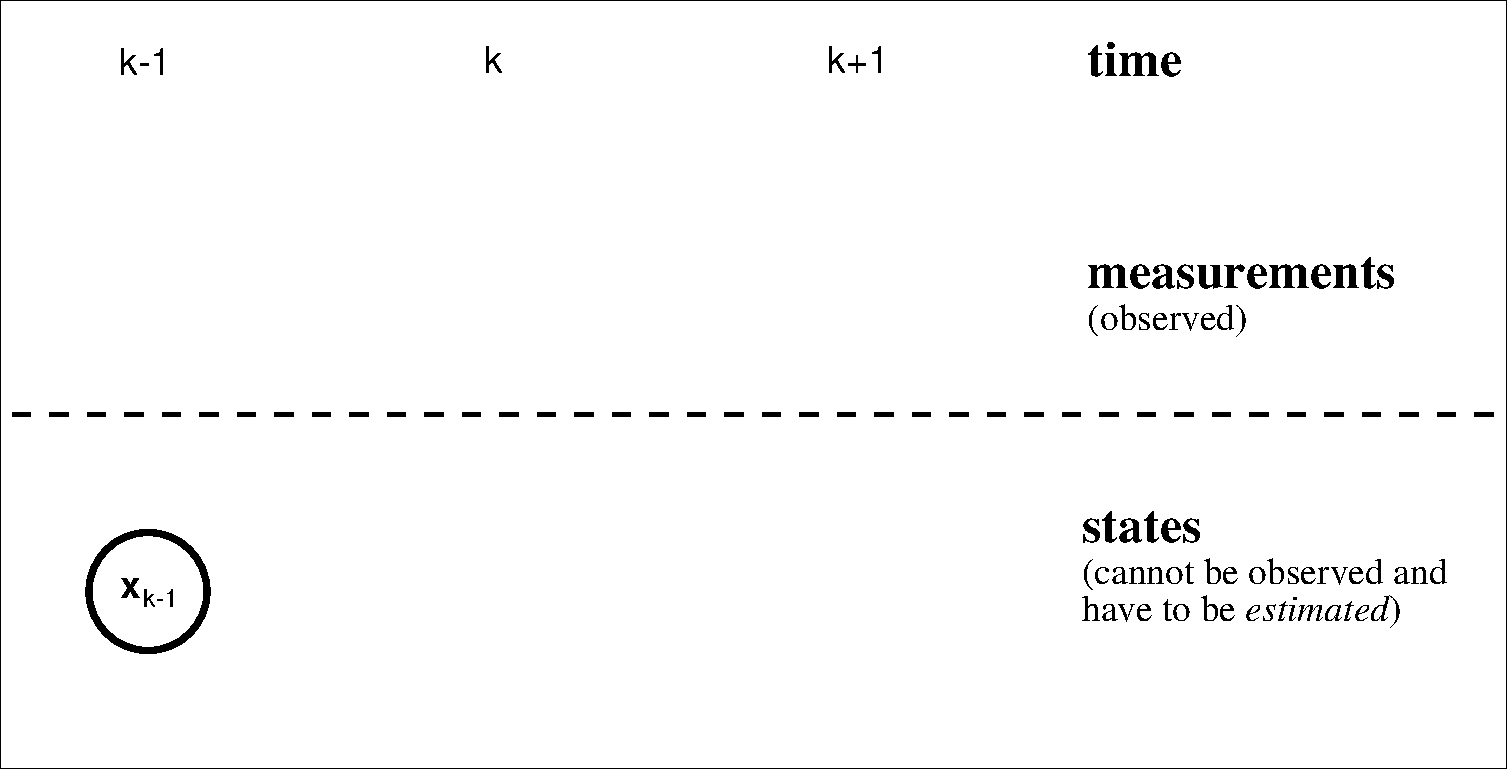
\includegraphics[width=.99\textwidth]{BucSystem1}


\newpage
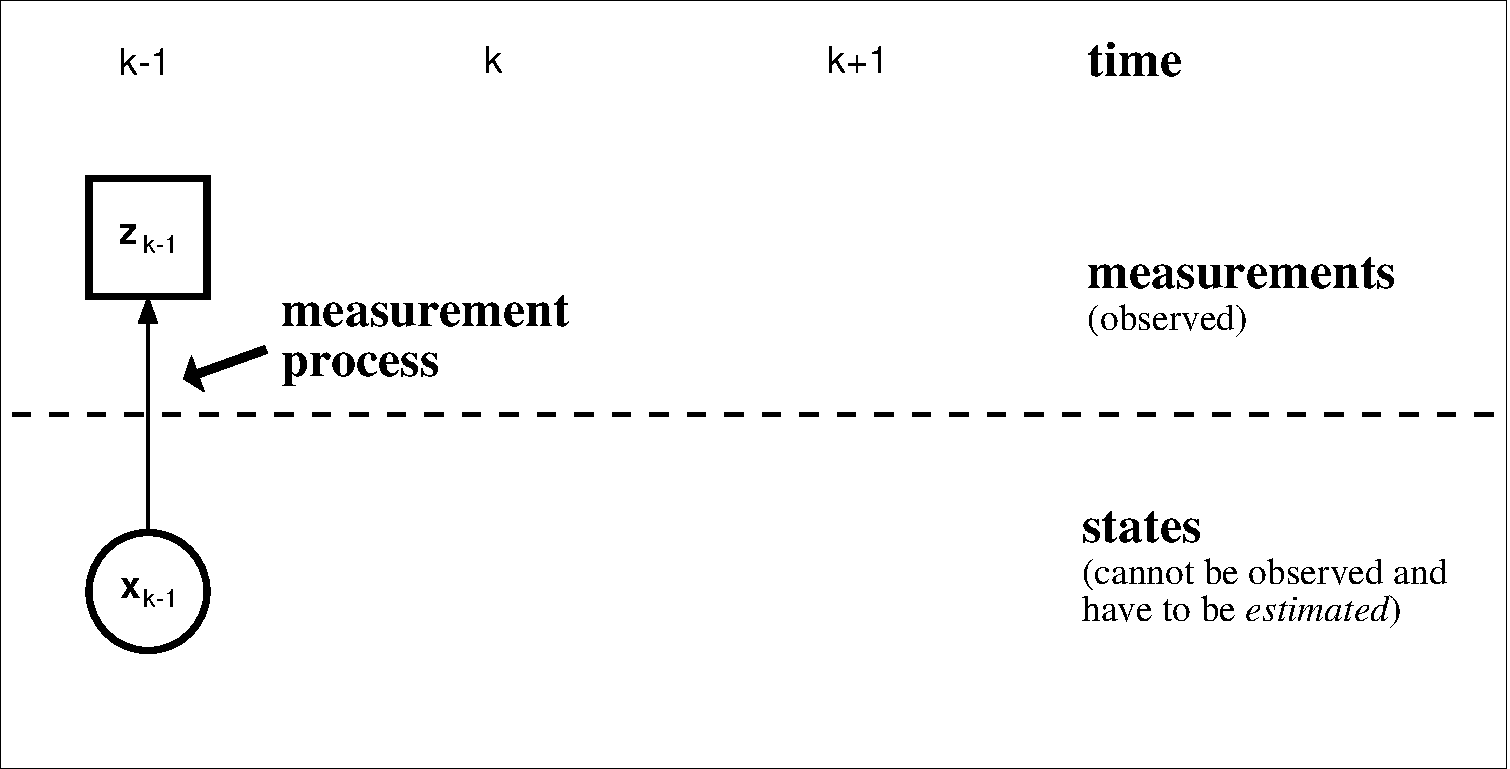
\includegraphics[width=.99\textwidth]{BucSystem2}


\newpage
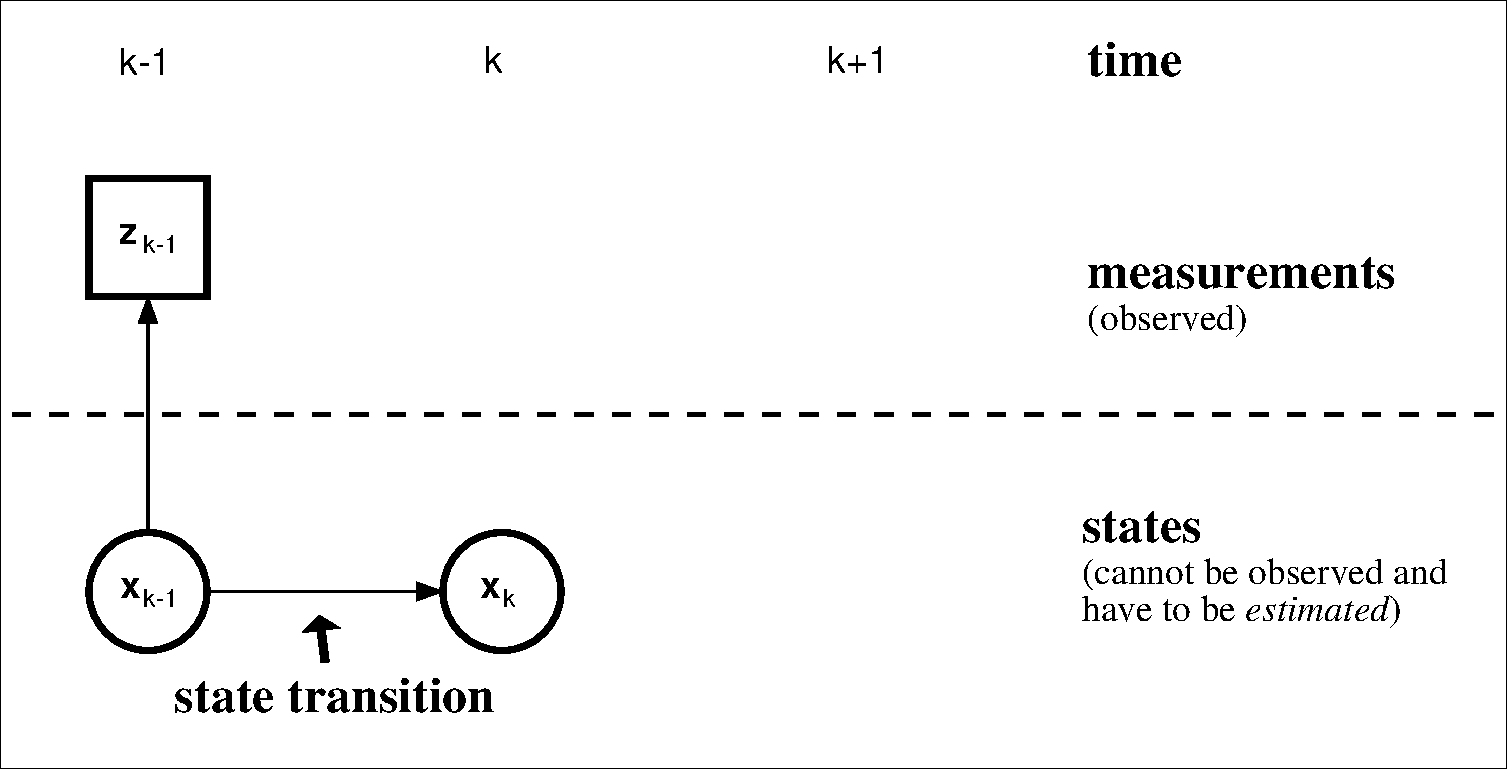
\includegraphics[width=.99\textwidth]{BucSystem3}


\newpage
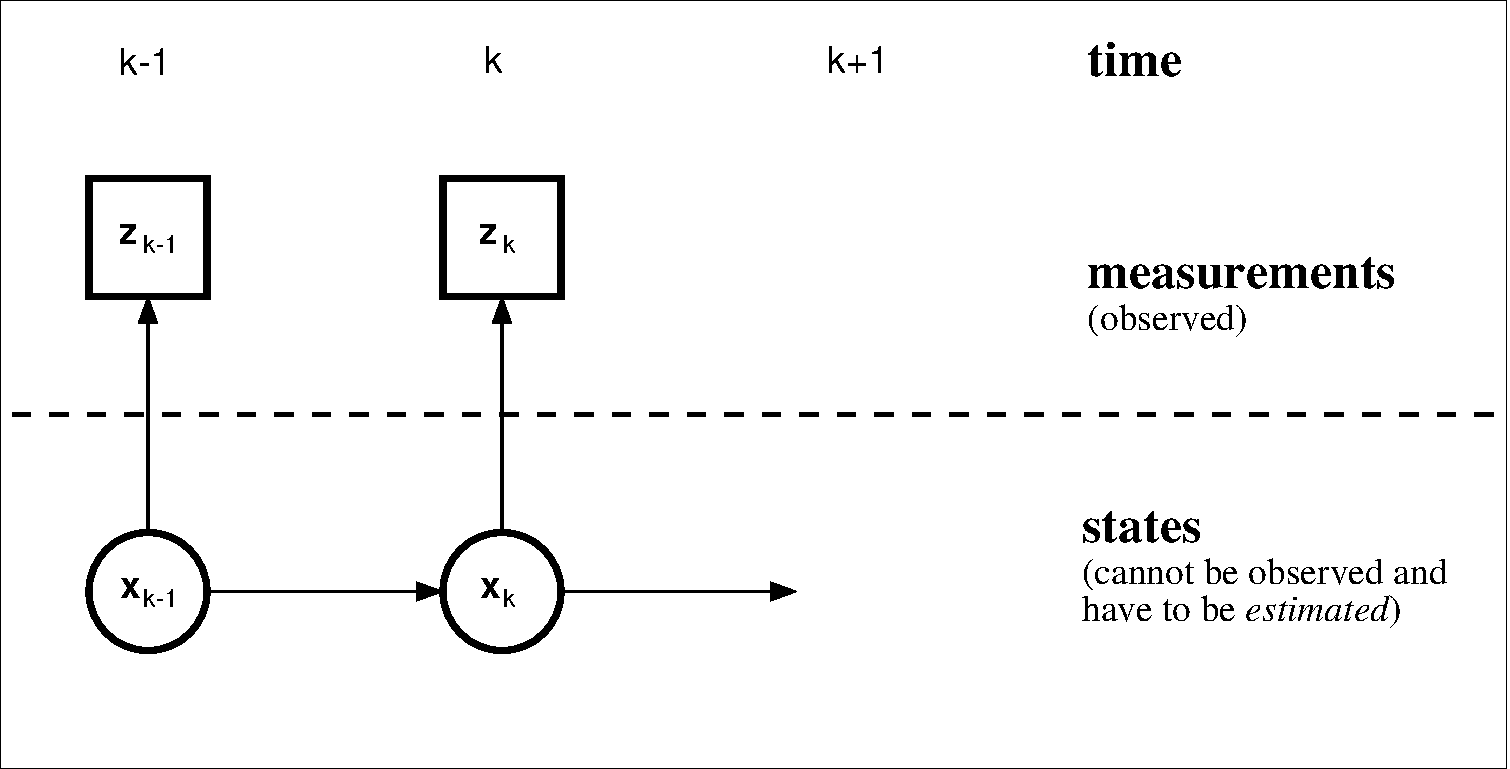
\includegraphics[width=.99\textwidth]{BucSystem4}


\newpage
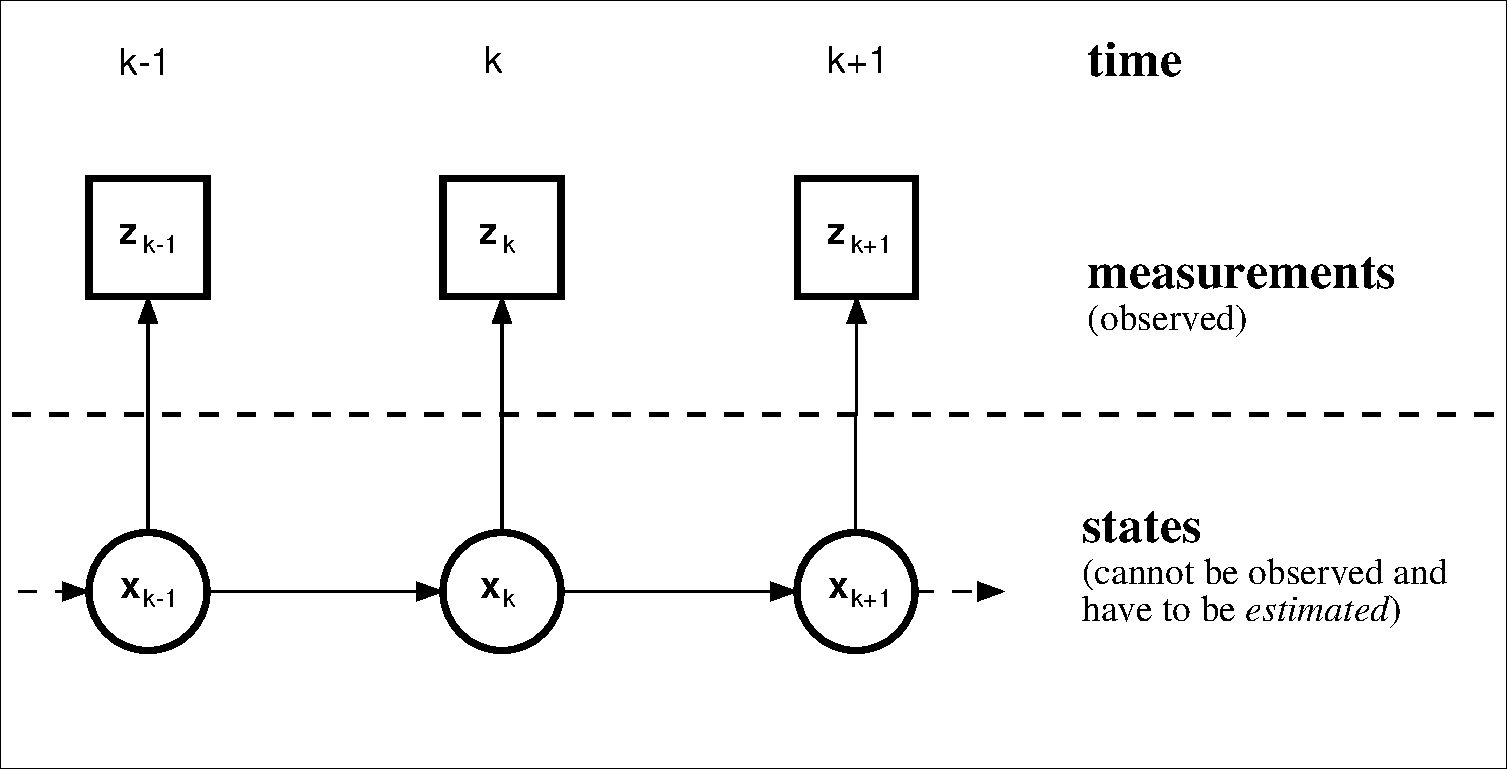
\includegraphics[width=.99\textwidth]{BucSystem5}


\newpage
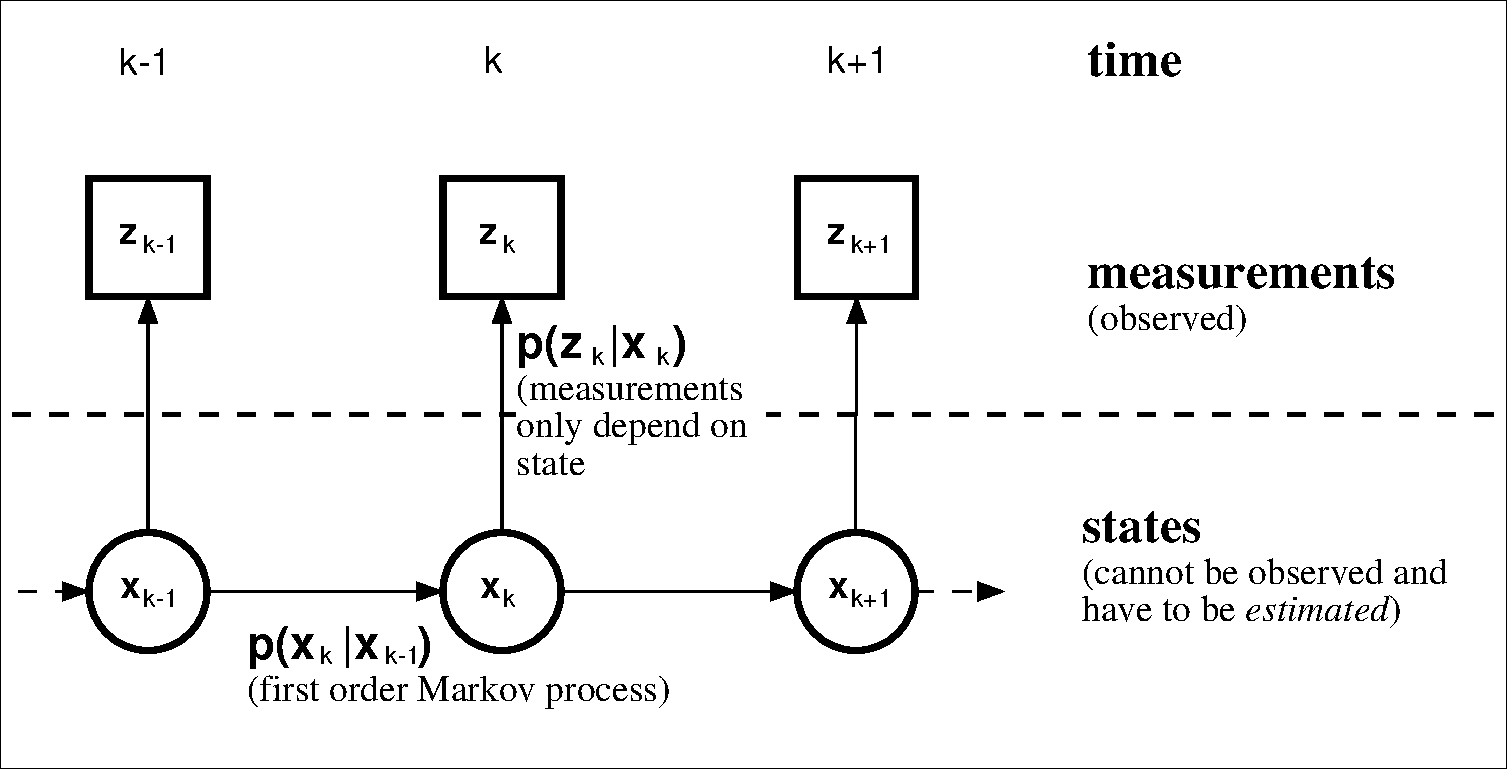
\includegraphics[width=.99\textwidth]{BucSystem6}

Assumptions:

The observations are conditionally independent given the state:
$p(\vz_k|\vx_k)$.

Hidden Markov Model (HMM):\\
$p(\vx_0)$ given and $p(\vx_k|\vx_{k-1})$ defines state transition probability for $k \ge 1$.


\newpage
\pagenumbering{restore}




\section{Bayesian Filters}


\subsection{Estimating the Posterior}

Bayesian approach: We attempt to construct the posterior pdf of
the state given all measurements.

$\Rightarrow$ can be termed a complete solution to the estimation
problem because all available information is used; from the pdf,
an optimal estimate can theoretically be found for any criterion.

in detail: We seek estimates of $\vx_k$ based on all available
measurements up to time $k$ (abbreviated as $\vz_{1:k}$) by
constructing the posterior $p(\vx_k|\vz_{1:k})$.

Assumption: initial state pdf (prior) $p(\vx_0)$ is given



\newpage
\subsection{The Use of Knowing the Posterior}

Let $f_k : \Realnumbers^{(k+1)\times n_x} \to \Realnumbers$ be any
arbitrary (integrable) function that can depend
\begin{itemize}
  \item on all components of the state $\vx$
  \item on the whole trajectory in state-space
\end{itemize}

Examples: This function can be an estimator for the current state
or for future observations.

Then we can compute its expectation using
\[
    \Expect{f_k(\vx_{0:k})} = \int f(\vx_{0:k})
    p(\vx_{0:k}|\vz_{1:k}) d\vx_{0:k}
\]

MMSE estimate of state: $\hat{\vx} = \Expect{\vx_k}$. Other
estimates that can be computed: median, modes, confidence
intervals, kurtosis, \dots



\newpage
\subsection{Recursive Filters}

recursive filters (i.e. sequential update of previous estimate)
$\leftrightarrow$ batch processing (computation with all data in
one step)

not only faster: allow on-line processing of data (lower storage
costs, rapid adaption to changing signals characteristics)

essentially consist of two steps:
 \begin{description}
 \item[prediction step:] $p(\vx_{k-1}|\vz_{1:k-1}) \to
 p(\vx_{k}|\vz_{1:k-1})$ \\
 (usually deforms / translates / spreads state pdf due to noise)
 \item[update step:] $p(\vx_{k}|\vz_{1:k-1}),\vz_k \to p(\vx_{k}|\vz_{1:k})$\\
 (combines likelihood of current measurement with predicted state;
 usually concentrates state pdf)
 \end{description}


\newpage
\subsection{General Prediction-Update Framework}

Assume that pdf $p(\vx_{k-1}|\vz_{1:k-1})$ is available at time
$k-1$.

Prediction step: (using Chapman-Kolmogoroff equation)
\begin{equation}
 \label{eq:predict}
  p(\vx_k|\vz_{1:k-1}) = \int
  p(\vx_k|\vx_{k-1}) p(\vx_{k-1}|\vz_{1:k-1}) d\vx_{k-1}
\end{equation}
This is the prior of the state $\vx_k$ at time $k$ \emph{without
knowledge of the measurement $\vz_k$}, i.e. the probability
\emph{given only previous measurements}.

Update step: (compute posterior pdf from
predicted prior pdf and new measurement)
\begin{equation}
 \label{eq:update}
  p(\vx_k|\vz_{1:k}) = \frac{p(\vz_k|\vx_k)p(\vx_k|\vz_{1:k-1})}{p(\vz_{k}|\vz_{1:k-1})}
\end{equation}





\newpage
\pagenumbering{incremental}

\def\temp{Let us prove formula (\ref{eq:update}) (just in order to train calculations
with joint and conditional probabilities\dots)}
\temp
\begin{eqnarray*}
    && \hspace*{75mm} \\[-5mm]
    && \textcolor{blue}{p(\vx_k|\vz_{1:k})} \\
    &&= \frac{\textcolor{blue}{p(\vz_{1:k}|\vx_k)p(\vx_k)}}{\textcolor{blue}{p(\vz_{1:k})}}
\end{eqnarray*}
(Bayes rule)


\newpage
\temp
\begin{eqnarray*}
    && \hspace*{75mm} \\[-5mm]
    && p(\vx_k|\vz_{1:k}) \\
    &&= \frac{\textcolor{blue}{p(\vz_{1:k}|\vx_k)}p(\vx_k)}{\textcolor{dgreen}{p(\vz_{1:k})}} \\
    &&= \frac{\textcolor{blue}{p(\vz_{k},\vz_{1:k-1}|\vx_k)}p(\vx_k)}{\textcolor{dgreen}{p(\vz_{k},\vz_{1:k-1})}}
\end{eqnarray*}
(separate $p(\vz_{1:k})$ into $p(\vz_k,\vz_{1:k-1})$)


\newpage
\temp
\begin{eqnarray*}
    && \hspace*{75mm} \\[-5mm]
    && p(\vx_k|\vz_{1:k}) \\
    &&= \frac{p(\vz_{1:k}|\vx_k)p(\vx_k)}{p(\vz_{1:k})} \\
    &&= \frac{\textcolor{blue}{p(\vz_{k},\vz_{1:k-1}|\vx_k)}p(\vx_k)}{\textcolor{dgreen}{p(\vz_{k},\vz_{1:k-1})}} \\
    &&= \frac{\textcolor{blue}{p(\vz_{k}|\vz_{1:k-1},\vx_k)p(\vz_{1:k-1}|\vx_k)}
        p(\vx_k)}{\textcolor{dgreen}{p(\vz_{k}|\vz_{1:k-1})p(\vz_{1:k-1})}}
\end{eqnarray*}
(factorize joint probability: $p(a,b|c) = p(a|b,c)\cdot p(b|c)$
and $p(a,b) = p(a|b)\cdot p(b)$)


\newpage
\temp
\begin{eqnarray*}
    && \hspace*{75mm} \\[-5mm]
    && p(\vx_k|\vz_{1:k}) \\
    &&= \frac{p(\vz_{1:k}|\vx_k)p(\vx_k)}{p(\vz_{1:k})} \\
    &&= \frac{p(\vz_{k},\vz_{1:k-1}|\vx_k)p(\vx_k)}{p(\vz_{k},\vz_{1:k-1})} \\
    &&= \frac{p(\vz_{k}|\vz_{1:k-1},\vx_k)\textcolor{blue}{p(\vz_{1:k-1}|\vx_k)}
        p(\vx_k)}{p(\vz_{k}|\vz_{1:k-1})p(\vz_{1:(k-1}))} \\
    &&= \frac{p(\vz_{k}|\vz_{1:k-1},\vx_k)\textcolor{blue}{p(\vx_k|\vz_{1:k-1})p(\vz_{1:k-1})}
        p(\vx_k)}{p(\vz_{k}|\vz_{1:k-1})p(\vz_{1:k-1})\textcolor{blue}{p(\vx_k)}}
\end{eqnarray*}
(Bayes rule)


\newpage
\temp
\begin{eqnarray*}
    && \hspace*{75mm} \\[-5mm]
    && p(\vx_k|\vz_{1:k}) \\
    &&= \frac{p(\vz_{1:k}|\vx_k)p(\vx_k)}{p(\vz_{1:k})} \\
    &&= \frac{p(\vz_{k},\vz_{1:k-1}|\vx_k)p(\vx_k)}{p(\vz_{k},\vz_{1:k-1})} \\
    &&= \frac{p(\vz_{k}|\vz_{1:k-1},\vx_k)p(\vz_{1:k-1}|\vx_k)
        p(\vx_k)}{p(\vz_{k}|\vz_{1:k-1})p(\vz_{1:(k-1}))} \\
    &&= \frac{\textcolor{blue}{p(\vz_{k}|\vz_{1:k-1},\vx_k)}p(\vx_k|\vz_{1:k-1})\textcolor{dgreen}{p(\vz_{1:k-1})
        p(\vx_k)}}{p(\vz_{k}|\vz_{1:k-1})\textcolor{dgreen}{p(\vz_{1:k-1})p(\vx_k)}} \\
    &&= \frac{\textcolor{blue}{p(\vz_k|\vx_k)}p(\vx_k|\vz_{1:k-1})}{p(\vz_{k}|\vz_{1:k-1})}
\end{eqnarray*}
(independence of observations; cancelling out terms)



\newpage
\pagenumbering{restore}

\subsection{The Structure of the Update Equation}

\begin{eqnarray*}
  p(\vx_k|\vz_{1:k}) &=& \frac{p(\vz_k|\vx_k)\cdot p(\vx_k|\vz_{1:k-1})}{p(\vz_{k}|\vz_{1:k-1})}
  \\[1.5ex]
  \mbox{posterior} &=& \frac{\mbox{likelihood}\cdot\mbox{prior}}{\mbox{evidence}}
\end{eqnarray*}

prior: given by prediction equation

likelihood: given by observation model

evidence: the normalizing constant in the denominator
\[
  p(\vz_{k}|\vz_{1:k-1}) = \int p(\vz_k|\vx_k)p(\vx_k|\vz_{1:k-1}) d\vx_k
\]




\newpage

This theoretically allows an optimal Bayesian solution (in the
sense of computing the posterior pdf).

\mybox{Problem: only a conceptual solution; integrals are not
tractable.}

But: in some restricted cases, an optimal solution is possible.
Two optimal solutions (under restrictive assumptions):
\begin{itemize}
  \item (standard) Kalman filter
  \item grid-based filter
\end{itemize}



\section{Kalman Filter}

\subsection{Introduction}

Assumptions:
\begin{itemize}
  \item posterior at time $k-1$, i.e. $p(\vx_{k-1}|\vz_{k-1})$, is Gaussian
  \item dynamic system characterized by
  \begin{eqnarray*}
    &{\color{StateColor}\vx_k} = {\color{StateFuncColor}\MF_k}{\color{StateColor}\vx_{k-1}}
    +
    {\color{StateFuncColor}\MG_k}{\color{StateNoiseColor}\vv_{k-1}}&
    \\
    &{\color{MeasColor}\vz_k} = {\color{MeasFuncColor}\MH_k}{\color{StateColor}\vx_k}
    +
    {\color{MeasFuncColor}\MJ_k}{\color{MeasNoiseColor}\vn_k}&
  \end{eqnarray*}
  \item both noise vectors Gaussian (covariance matrices are $\MQ_{k-1}$ and $\MR_k$)
\end{itemize}
Then new posterior $p(\vx_{k}|\vz_{k})$ is Gaussian, too, and can
be computed using simple linear equations.

optimal solution, but \emph{highly restrictive} assumptions must hold


%\newpage
\subsection{Prediction Equation}

At time $k-1$: $p(\vx_{k-1}|\vz_{1:k-1}) = {\cal N}(\vm_{k-1|k-1}, \MP_{k-1|k-1})$

Inserting into (\ref{eq:predict}) yields
\[
  p(\vx_k|\vz_{1:k-1}) = {\cal N}(\vm_{k|k-1}, \MP_{k|k-1})
\]
with
\[
  \vm_{k|k-1} = \MF_k\vm_{k-1|k-1}
\]
and
\[
  \MP_{k|k-1} = \MG_{k}\MQ_{k-1}\MG_{k}^T + \MF_k\MP_{k-1|k-1}\MF_k^T
\]



\newpage
\subsection{Update Equation}

Inserting into (\ref{eq:update}) yields
\[
  p(\vx_k|\vz_{1:k}) = {\cal N}(\vm_{k|k}, \MP_{k|k})
\]
with
\[
  \vm_{k|k} = \vm_{k|k-1} + \MK_k (\vz_k - \underbrace{\MH_k\vm_{k|k-1}}_{\mbox{\small estimated }\hat{\vz}_k})
\]
and
\[
  \MP_{k|k} = \MP_{k|k-1} - \MK_k\MH_k\MP_{k|k-1}
\]
Kalman Gain:
\[
  \MK_k = \MP_{k|k-1}\MH_k^T(\underbrace{\MH_k\MP_{k|k-1}\MH_k^T + \MJ_k\MR_k\MJ_k^T}_{\mbox{$\Cov{\hat{\vz}_k}$}})^{-1}
\]






\section{Grid-Based Filter}


\subsection{Introduction}

Assumptions:
\begin{itemize}
  \item state space is discrete
  \item number of different states ($N_s$) is limited \\
  {\footnotesize (Note: implicitly includes discreteness)}
\end{itemize}

Suppose at time $k-1$ we have states $\vx^i$ with
$i=1,\ldots,N_s$. Conditional probability of these states:
\[
  Pr(\vx_{k-1} = \vx^i|\vz_{1:k-1}) = w_{k-1|k-1}^i
\]
Then the (old) posterior at time $k-1$ is given by:
\[
  p(\vx_{k-1}|\vz_{1:k-1}) = \sum_{i=1}^{N_s} w_{k-1|k-1}^i \; \delta(\vx_{k-1}-\vx^i)
\]

\newpage

\subsection{Results (Summary)}

Both the (new) prior and the (new) posterior have the same
structure: a sum of weighted Dirac peaks:

\[
  p(\vx_{k}|\vz_{1:k-1}) = \sum_{i=1}^{N_s} w_{k|k-1}^i \; \delta(\vx_{k-1}-\vx^i)
\]
\[
  p(\vx_{k}|\vz_{1:k}) = \sum_{i=1}^{N_s} w_{k|k}^i \; \delta(\vx_{k-1}-\vx^i)
\]

Note: extension to different sets of states for each time step
\[
  \{\vx^i\}: i=1,\ldots,N_s \quad\longrightarrow\quad \{\vx^i_k\}: i=1,\ldots,N_{s,k}
\]
with time-varying index $k$ is easily possible; the `allowed'
states need not be constant.



\newpage
\subsection{Prediction Equation (in Detail)}

Inserting into (\ref{eq:predict}) yields
\begin{eqnarray*}
  p(\vx_k|\vz_{1:k-1})
  &=& \sum_{i=1}^{N_s} \sum_{j=1}^{N_s} w_{k-1|k-1}^j
      p(\vx^i|\vx^j) \delta(\vx_{k-1}-\vx^i)\\
  &=& \sum_{i=1}^{N_s} w_{k|k-1}^i \delta(\vx_{k-1}-\vx^i)
\end{eqnarray*}
where $w_{k|k-1}^i = \sum_{j=1}^{N_s} w_{k-1|k-1}^j
p(\vx^i|\vx^j)$

\bigskip
\mybox{(new) prior weights = old posterior weights,\\
reweighted using state transition probabilities}




\newpage
\subsection{Update Equation (in Detail)}

Inserting into (\ref{eq:update}) yields
\[
  p(\vx_k|\vz_{1:k}) = \sum_i^{N_s} w_{k|k}^i \delta(\vx_{k-1}-\vx^i)
\]
where $w_{k|k}^i = \frac{w_{k|k-1}^i
p(\vz_{k}|\vx^i)}{\sum_j^{N_s} w_{k|k-1}^j
p(\vz_{k}|\vx^j)}$.

Note: denominator only needed for normalization

\bigskip
\mybox{posterior weights = prior weights, reweighted using
likelihoods}





\section{Particle Filter}


\subsection{Suboptimal Approximations}

If we want to preserve Kalman filter principle\dots
\begin{itemize}
  \item Extended Kalman Filter (EKF)
  \item Unscented Kalman Filter (UKF)
\end{itemize}
...we get better results, \mybox{BUT: \emph{we cannot get rid off
Gaussian approximations}}

\newpage

EKF / UKF: \mybox{All these approaches fail if we have
\begin{itemize}
  \item bimodal / multimodal pdfs
  \item heavily skewed pdfs
\end{itemize}
}

We need a more general scheme to tackle these problems.


\newpage
\subsection{Particle Filter -- General Concept}

Many different names (do you remember the
\href{#section.1}{introduction}?) but the general concept is
rather simple:

\mybox{PARTICLE FILTER:

If we cannot solve the integrals required for a Bayesian recursive
filter analytically \dots we represent the posterior probabilities
by a set of randomly chosen weighted samples.}

Note: ``randomly chosen'' $\equiv$ ``Monte Carlo'' \\
(we are playing roulette / throwing the dice)

Increasing number of samples $\Rightarrow$ (almost sure)
convergence to true pdf



\newpage
\subsection{Sequential Importance Sampling (SIS)}

SIS is the basic framework for most particle filter algorithms.
Let
\begin{eqnarray*}
    \{\vx_{0:k}^i\} &:& \mbox{set of support points
    (samples, particles)} \\
    && i = 1,\ldots,N_s \\
    && \mbox{(whole trajectory for each particle!)} \\
    w_{k}^i &:& \mbox{associated weights, normalized to $\sum_i w_k^i = 1$}
\end{eqnarray*}
Then:
\[
    p(\vx_k|\vz_{1:k}) \approx \sum_{i=1}^{N_s} w_k^i \delta(\vx_{0:k} - \vx^i_{0:k})
\]
(discrete weighted approximation to the true posterior)


\newpage
\subsection*{SIS (continued)}

Usually we cannot draw samples $\vx_k^i$ from $p(\cdot)$ directly.
Assume we sample directly from a (different) \emph{importance
function} $q(\cdot)$. Our approximation is still correct (up to
normalization) if
\[
    w_k^i \propto \frac{p(\vx^i_{0:k}|\vz_{1:k})}{q(\vx^i_{0:k}|\vz_{1:k})}
\]
\mybox{The trick: we can choose $q(\cdot)$ freely!}

If the importance function is chosen to factorize such that
\[
    q(\vx_{0:k}|\vz_{1:k}) = q(\vx_{k}|\vx_{0:k-1},\vz_{1:k})\;q(\vx_{0:k-1}|\vz_{1:k-1})
\]
then one can augment old particles $\vx^i_{0:k-1}$ by $\vx_k \sim
q(\vx_{k}|\vx_{0:k-1},\vz_{1:k})$ to get new particles
$\vx^i_{0:k}$.


\newpage
\subsection*{SIS (continued)}

Weight update (after some lengthy computations\dots):
\begin{equation}
 \label{eq:WeightUpdate}
    w_k^i = w^i_{k-1}
    \frac{p(\vz_k|\vx^i_k)\,p(\vx^i_{k}|\vx^i_{k-1})}{q(\vx^i_{k}|\vx^i_{0:k-1},\vz_{1:k})}
\end{equation}
Furthermore, if $q(\vx_{k}|\vx_{0:k-1},\vz_{1:k}) =
q(\vx_{k}|\vx_{k-1},\vz_{1:k})$\\
(only dependent on \emph{last} state and observations):
\[
    p(\vx|\vz_{1:k}) \approx \sum_{i=1}^{N_s} w_k^i \,\delta(\vx_k -
    \vx_k^i)
\]
(and we need not preserve trajectories $\vx^i_{0:k-1}$ and history
of observations $\vz_{1:k-1}$)


\newpage
\subsection{SIS Algorithm -- Pseudo Code}

\mycodebox{
 [\codemath{\{\vx^i_k,w^i_k\}_{i=1}^{N_s}}] = SIS(\codemath{\{\vx^i_{k-1},w^i_{k-1}\}_{i=1}^{N_s}},
 \codemath{\vz_k}) \\
 \hspace*{7mm} FOR \codemath{i} = \codemath{1} : \codemath{N_s} \\
 \hspace*{14mm}   \codetext{draw} \codemath{\vx_k^i \sim q(\vx_{k}|\vx^i_{k-1},\vz_{k})} \\
 \hspace*{14mm}   \codetext{update weights according to (\ref{eq:WeightUpdate})} \\
 \hspace*{7mm} END FOR \\
 \hspace*{7mm} \codetext{normalize weights to} \codemath{\sum_{i=1}^{N_s} w_k^i = 1}
}



\newpage
\subsection{PROBLEM: Degeneracy Problem}

Problem with SIS approach: after a few iterations, most particles
have negligible weight (the weight is concentrated on a few
particles only)

Counter measures:
\begin{itemize}
  \item brute force: many, many samples $N_s$
  \item good choice of importance density
  \item resampling
\end{itemize}

Note: amount of degeneracy can be estimated based on variance of
weights [Liu 1996].



\newpage
\subsection{Optimal Impotance Density:}

It can be shown that the optimal importance density is given by
\[
    q(\vx_k|\vx_{k-1},\vz_k)_{opt} = p(\vx_k|\vx_{k-1},\vz_k)
\]
Then
\[
    w^i_k = w^i_{k-1} \int p(\vz_k|\vx'_k) p(\vx'_k|\vx^i_{k-1})
    d\vx'_k
\]
Two major drawbacks: usually neither sampling from $q_opt$ nor
solving the integral in $w^i_k$ is possible\dots (but in some
special cases, it works)

Other alternative which is often convenient: \\
$q(\cdot) = p(\vx_k|\vx_{k-1})$ (prior). Easy to implement, but does not take
measurements into account.



\newpage
\subsection{Resampling Approaches}

Basic idea of resampling:
 \mybox{Whenever degeneracy rises above threshold: replace old set of samples
 (+ weights) with new set of samples (+ weights), such that sample density
 better reflects posterior pdf.}

This eliminates particles with low weight and chooses more
particles in more probable regions.

Complexity: possible in $O(N_s)$ operations


\newpage
The resampling principle:

\begin{center}
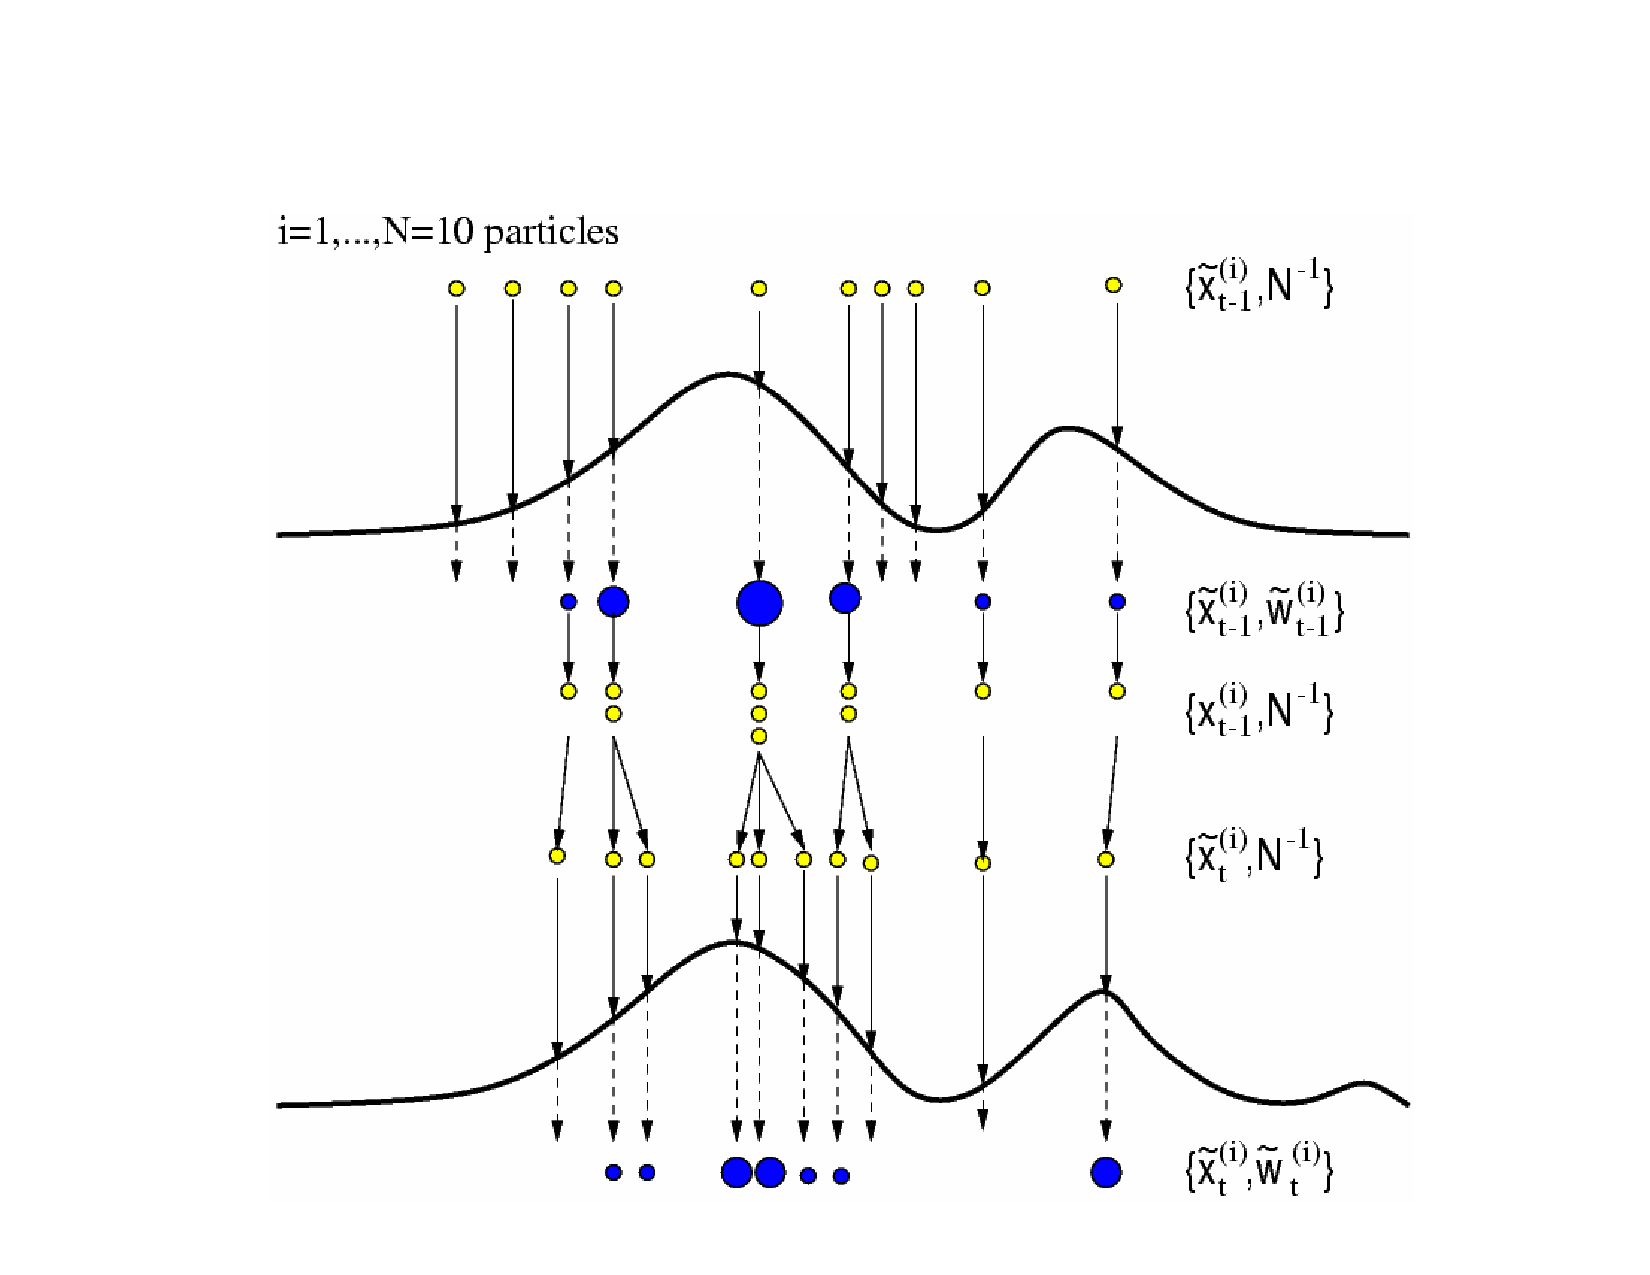
\includegraphics[width=0.8\linewidth]{BucResampling}
\end{center}

(graphics taken from Van der Merwe et al.)



\newpage
\subsection{General Particle Filter -- Pseudo Code}

\mycodebox{
 [\codemath{\{\vx^i_k,w^i_k\}_{i=1}^{N_s}}] = PF(\codemath{\{\vx^i_{k-1},w^i_{k-1}\}_{i=1}^{N_s}},
 \codemath{\vz_k}) \\
 \hspace*{7mm} FOR \codemath{i} = \codemath{1} : \codemath{N_s} \\
 \hspace*{14mm}   \codetext{draw} \codemath{\vx_k^i \sim q(\vx_{k}|\vx^i_{k-1},\vz_{k})} \\
 \hspace*{14mm}   \codetext{update weights according to (\ref{eq:WeightUpdate})} \\
 \hspace*{7mm} END FOR \\
 \hspace*{7mm} \codetext{normalize weights to} \codemath{\sum_{i=1}^{N_s} w_k^i = 1}\\
 \hspace*{7mm} IF \codetext{degeneracy too high} \\
 \hspace*{14mm}   \codetext{resample} \codemath{\{\vx^i_k,w^i_k\}_{i=1}^{N_s}} \\
 \hspace*{7mm} END IF
}




\newpage
\subsection{PROBLEM: Loss of Diversity}

No degeneracy problem but new problem arises:
%
\mybox{Particles with high weight are selected more and more
often, others die out slowly

$\Rightarrow$ \emph{loss of diversity} or \emph{sample
impoverishment}}

For small process noise, all particles can collapse into a single
point within a few iterations.

Other problem: resampling limits the ability to parallelize
algorithm.



\newpage
\subsection{Other Particle Filter Variants}


Methods to counteract loss of diversity and degeneracy problem:
\begin{itemize}
  \item resample-move algorithm
  \item regularization
  \item Rao-Blackwellisation
  \item multiple Monte-Carlo
\end{itemize}

Other particle filter variants found in the literature:
\begin{itemize}
  \item sampling importance resampling (SIR)
  \item auxiliary sampling importance resampling (ASIR)
  \item regularized particle filter (RPF)
  \item \dots
\end{itemize}




\section{Experiments}

see videos...



\section{Summary}

First of all: what I did \emph{not} talk about\dots
\begin{itemize}
  \item speed of convergence
  \item number of samples needed
  \item complexity issues / tricks for speed-up of algorithms
  \item advanced particle filter variants in detail
\end{itemize}


$\Rightarrow$ refer to the literature if you want to know more



\newpage
Advantages of particle filters (PFs):
\begin{itemize}
  \item can deal with non-linearities
  \item can deal with non-Gaussian noise
  \item can be implemented in $O(N_s)$
  \item mostly parallelizable
  \item easy to implement
  \item in contrast to HMM filters (state-space discretized to $N$ fixed
  states) : PFs focus adaptively on probable regions of state-space
\end{itemize}



\newpage
{\bfseries\Large Thesis:}

\myboxii{If you want to solve a filtering problem, then particle
filters are the best filters you can use, much better than e.g.
Kalman filters.}

\textcolor{dgreen}{\bfseries Right} or \textcolor{red}{\bfseries wrong}?


\newpage

\textcolor{red}{\bfseries WRONG}!

Particle filters include a random element; they only convergence
to the true posterior pdf (almost surely) if $N_s \to \infty$.

Therefore: \emph{If the assumptions for Kalman filters or
grid-based filters are valid, no PF can outperform them!}

Additionally: depending on the dynamic model, Gaussian sum
filters, unscented Kalman filters or extended Kalman filters may
produce satisfactory results at lower computational cost.

(But you should at least try a PF; it is usually better than other
suboptimal methods!)




\newpage
PF approaches proved their usefulness in a variety of
applications.

But:
\begin{itemize}
  \item choice of importance function $q(\cdot)$ is crucial in PF
  design
  \item large sample number $N_s$ increases computational effort
  \item potential problems: \emph{degeneracy} and \emph{loss of diversity}
\end{itemize}

\mybox{If these points are taken into account, then particle
filters are an extremely powerful tool for filtering /
estimation.}

(``black box usage'' vs ``know what you're doing!'')





\newpage
\vspace*{2cm}


{\Huge Thank you!}

\vspace{1.3cm}

\begin{raggedleft}
  \footnotesize
  This presentation was made with \LaTeX.\\
  (try to write Bucure\c{s}ti in Powerpoint\dots)\\
\end{raggedleft}



\end{document}
